\section{Research Plan and Methodology} \label{sec:rep}

This \xxx project tackles concurrency attacks with a thorough, systematic 
methodology. To this end, this section presents three objectives in this 
section, including a general, rigorous concurrency attack model 
(\S\ref{sec:model}), a systematic concurrency attack detection approach 
(\S\ref{sec:detect}) by leveraging this model, and a runtime defense 
infrastructure (\S\ref{sec:defense}). Each objective includes our preliminary 
results. Finally, this section describes our research plan (\S\ref{sec:plan}).

\vspace{-.15in}\subsection{Objective 1: Modeling Concurrency Attacks} 
\label{sec:model}\vspace{-.075in}

% P1: as mentioned in background, a key reason is thread interleavings, 
% so we need to reason about the general patterns we have. Or we say our 
% methodology is just like pattern matching.
As mentioned in \S\ref{sec:background}, state-of-the-art lacks a rigorous model 
for concurrency attacks. Specifically, people lack understanding on how 
concurrency bugs propagate to vulnerable instructions in source code. This 
section first gives two concurrency attack examples our preliminary study 
successfully constructed (\S\ref{sec:examples}), and then proposes 
our model (\S\ref{sec:attack-phase}).

\vspace{-.15in}\subsubsection{Concurrency Attacks Examples In Our Preliminary 
Study} 
\label{sec:examples}\vspace{-.075in}

Figure~\ref{fig:libsafe} shows the code of a concurrency attack in 
\libsafe~\cite{libsafe}, a popular stack overflow protection library. \libsafe
provides its own safe memory and string operations functions. For instance, the 
\texttt{libsafe\_strcpy()} function checks whether a stack variable is passed 
in as the function argument \texttt{dest} before it calls the actual 
\texttt{strcpy()}. If a program receives a kill signal, Libsafe's internal 
thread (Thread 1) sets a global variable \texttt{dying}, then security checks 
are disabled in \texttt{libsafe\_strcpy()}. Unfortunately, \texttt{dying} was 
not protected by mutex locks. In our study, we triggered a data race on this 
variable, bypassed the security check, and overflowed Thread 2's stack by 
passing malicious code to \texttt{dest}. Ironically, this \libsafe library is 
no longer ``safe" when facing concurrency attacks.

\begin{figure}[h]
\vspace{-.1in}
\centering
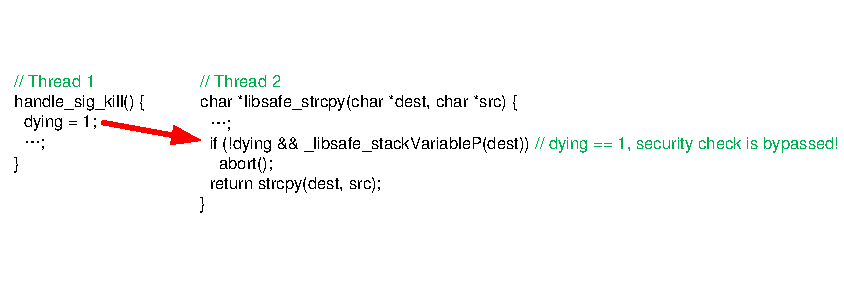
\includegraphics[width=0.8\columnwidth]{figures/libsafe}
\vspace{-.1in}
\caption{{A concurrency attack in the \libsafe security library.}} 
\label{fig:libsafe}
\vspace{-.15in}
\end{figure}

Figure~\ref{fig:apache} shows the code of a concurrency attack in 
the widely used \apache~\cite{apache} web server for maintaining users' HTTP 
pages. \apache spawns a number of threads, each serves a HTTP request. Each 
thread also records the request in a global log buffer in heap and flushes this 
buffer to a log file when the buffer is full. However, developers missed a 
mutex lock to protect this buffer, so the buffer can overflow and corrupt 
adjacent memory, including the log file's descriptor. In our study, we 
corrupted this descriptor and made \apache write a request record to mess up 
another user's HTTP page.

\begin{figure}[h]
\vspace{-.05in}
\centering
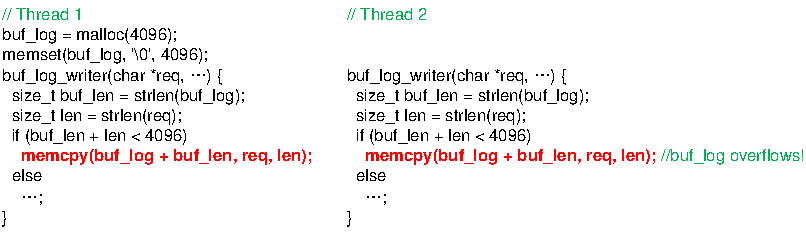
\includegraphics[width=0.8\columnwidth]{figures/apache}
\vspace{-.1in}
\caption{{A concurrency attack in the \apache web server.}} \label{fig:apache}
\vspace{-.15in}
\end{figure}



\vspace{-.15in}\subsubsection{Concurrency Attack Model} 
\label{sec:attack-phase}\vspace{-.075in}

Two key questions on modeling concurrency attacks are: (1) what are the common 
elments in concurrency attacks, and (2) how does the corrupted memory in a 
concurrency bug propagate to vulnerable instructions in source code? Since 
existing reliability tools (\S\ref{sec:others-work}) are already effective on 
detecting concurrency bugs, if our model can address these two questions, we 
can build software tools to effectively identify which concurrency bugs have 
the potential to lead to attacks, and we can safely ignore those don't.

% P3: pattern.
% \para{Three common elements.}
Although the two aforementioned examples appear to be diverse, we have 
identified three common elements in these concurrency attacks. First, it is 
necessary to have corrupted global memory (\eg, the \texttt{dying} variable in 
\libsafe, and the \texttt{buf\_len} buffer in \apache) caused by concurrency 
bugs. Second, it is necessary to have a vulnerable instruction (\eg, 
\texttt{strcpy()} or 
\texttt{setuid()}) to perform an attack. Third, the corrupted values in global 
memory must cause abnormal behavior on the vulnerable instructions. For 
example, the abnormal behavior in \libsafe is to leverage the corrupted 
memory to bypass the stack overflow check, an abnormal control-flow of the 
execution. For \apache, we directly corrupt (\ie, overflow) the buffer 
log, an abnormal data-flow of the execution.

% In sum, three common elements compose a concurrency attack model: corrupted 
% memory, security-sensitive operation, and impact (indirect or direct) from 
% the % memory to the operation.
% 
In addition to these two examples, the \noldattacks concurrency 
attacks in recent study~\cite{con:hotpar12} and the \nattacks ones our own 
preliminary study (\S\ref{sec:examples}) also have the three common elements. 
For the first element, these attacks have four types of concurrency bugs, 
including data races, atomicity violations, deadlocks, and order violations. 
For the second element, we have collected five types of vulnerable 
instructions, including memory operations (\eg, \texttt{strcpy()}), pointer 
deferences (\eg, when the pointer is NULL), privilege operations (\eg, 
\texttt{setuid()}), file operations (\eg, \texttt{access()}), and miscellaneous 
operations (\eg, \texttt{eval()} in shell scripts). For the third element, 
\S\ref{sec:detect} will propose our systematic detection approach to detect 
abnormal control-flow and data-flow of executions.

% PX: emphasis the contribution/potential value of this model.
% In a high level, this model treats a concurrency attack as a source-sink 
% model, 
% where a source is a corrupted global memory caused by a concurrency bug, and 
% a 
% sink is a security-sensitive operation. Then this model tracks the data flow 
% and control flow of the corrupted memory to the sensitive operations. Unlike 
% a 
% traditional model which only consider inputs as the source, our model 
% considers
% concurrency bugs as the the inputs. This model spurs several interesting 
% research questions. First, how do we track down the corrupted memory in the 
% middle of an execution? Second, given that concurrency bugs are not only just 
% one, how does our analysis handle multiple concurrency bugs (\eg, multiple 
% corrupted variables)? Third, given that not all security-sensitive operations 
% are indeed relevant to the source, how do we prune the irrelevant operations 
% soundly (\ie, without missing exploits)? In \S\ref{sec:detect}, we plan to 
% leverage this model to develop an effective detection approach, and our 
% preliminary work has shown promising results on addressing these research 
% questions.

% TBD: add a table on the list of concurrency bugs and the list of dangerous 
% operations.



% P5: how to handle unknow patterns? Just say patterns in our work may spur new 
% patterns. We will continue to find new patterns as well.
% P5: TBD.

% \subsubsection{Concurrency Attacks with Three Common Patterns}
% \label{sec:model-pattern}

% Goal 1: modeling.

\vspace{-.15in}\subsection{Objective 2: Detecting Concurrency Attacks in 
Testing Phase}\label{sec:detect}\vspace{-.075in}

% To detect the abnormal control-flow and data-flow between corrupted global 
% memory to vulnerable instructions, our approach takes program source code as 
% input, and it outputs whether this program has potential concurrency attacks. 
% This approach is mainly for program 
% developers to detect and fix potential attacks during the software 
% testing phase.

Our proposed detection approach is not only useful for developers to detect 
concurrency attacks during software testing phase, but also useful for 
analyzing concurrency bugs and their potential attacks in old releases of 
software programs. The reason is because even if 
concurrency bugs were already fixed in the latest software release, if 
concurrency attacks have occurred and hackers have broken in, simply fixing 
the bugs can not recover from the attacks (\S\ref{sec:examples}).

% For example, we studied a 
% few concurrency bugs in old Linux and BSD releases a few years ago, and their 
% attacks are still helpful because if attackers have broken in and gain root 
% privilege, simply fixing the 
% bugs or upgrading kernels can not remove the malicious root user.

\vspace{-.15in}\subsubsection{Workflow of \xxx's Detection Approach}
\label{sec:detect-arch}\vspace{-.075in}

We identify two major goals for our detection approach. First, a report should 
contain preconditions on program inputs so that developers can easily reproduce 
the concurrency attack. This goal is especially useful for developers to 
trigger attacks on rare inputs (\eg, nested \texttt{select} statements are 
required to trigger a concurrency attack to MySQL in our preliminary 
study study (\S\ref{sec:examples}).

Second, this approach should be precise in terms of having as few as false 
positives (reports but actually not a feasible attack) and false negatives 
(missing a real attack). To this end, this approach should capture only the 
data-flow and control-flow relevant for the propagation from corrupted memory 
to vulnerable instructions, and it should discard the irrelevant ones. 

We plan to achieve the first goal with \emph{symbolic 
execution} (\S\ref{sec:others-work}), a program analysis technique that 
systematically explore a program's execution paths to find bugs. Unlike normal 
execution which runs on a concrete input, this technique marks inputs (\eg, 
command line arguments) as ``symbolic" and tracks input preconditions 
on branch instructions (\eg, \texttt{if} and \texttt{while}) during the 
execution. If a branch instruction depends on inputs, symbolic execution forks 
a new execution, let the two executions go down different paths, and tracks 
input preconditions on each execution. This technique has shown to find new 
bugs in real-world systems programs~\cite{klee:osdi08}.

We plan to achieve the second goal with \emph{path slicing} 
(\S\ref{sec:others-work}). Given a 
trace of executed instructions and an essential instruction in this trace, 
path slicing starts from this essential instruction, goes backward the trace, 
and computes a subset of instructions that affect the reachability and operand 
values of this instruction. This path slicing technique has shown to compute 
compact input preconditions to block malicious inputs~\cite{castro:bouncer} and 
compute relevant instructions for programming rule 
violations~\cite{woodpecker:asplos13}.

By leveraging the symbolic execution and path slicing, the workflow of our 
detection approach is shown in Figure~\ref{fig:detection}. This approach takes 
program source code as input. Specifically, we compile the code into 
LLVM~\cite{llvm} instructions, a popular form of instructions for program 
anlysis tools. The symbolic execution engine marks a program input and bytes 
received from network as symbolic and explore program paths. For each execution, 
we collect all the the executed instructions as a trace, and run a race detector 
on the trace: if a concurrency bug is detected, we feed this trace to path 
slicer to see whether: (1) the trace may have contained a vulnerable 
instruction, or (2) this trace have any branch instruction that can lead to 
vulnerable instruction in the not executed branches. If the trace does not 
satisfy any of the two conditions, we then safely discard this trace.

% \begin{figure}[ht]
% \centering
% \vspace{-.1in}
% 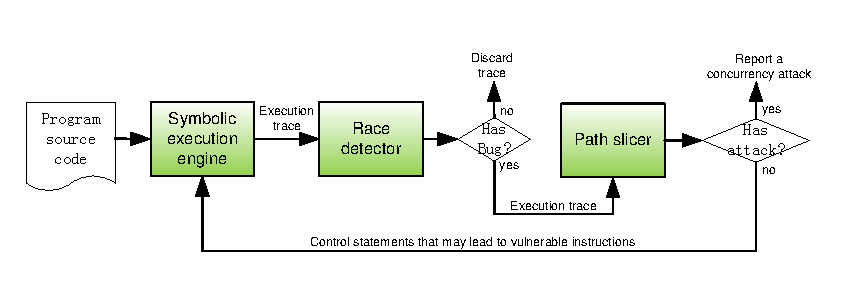
\includegraphics[width=0.8\columnwidth]{figures/detection}
% \vspace{-.1in}
% \caption{{Workflow of the concurrency attack detection scheme.}} 
% \label{fig:detection}
% \vspace{-.1in}
% \end{figure}

% \begin{figure}[ht]
% \centering
% % \begin{minipage}{.5\textwidth}
% \lgrindfile{code/explore.cpp.tex}
% % \end{minipage}
% \caption{{\em The \xxx search algorithm.}} \label{fig:alg}
% \end{figure}

% \input{code/explore.algo.tex}

% \begin{figure}[t]
% \begin{center}
% \subfloat[{\em Detection 
% workflow.}]{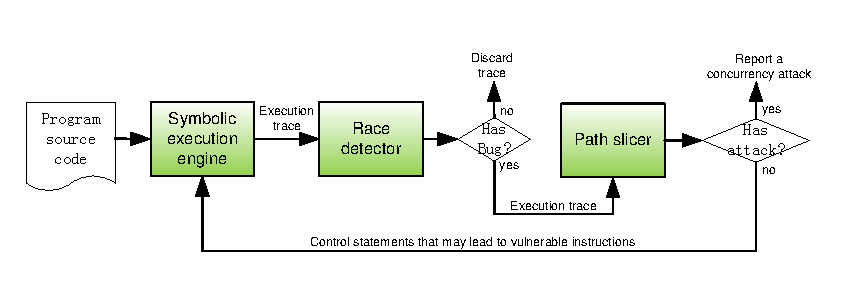
\includegraphics[width=.20\linewidth]{figures/detection}
% \label{fig:workflow}}
% \subfloat[{\em Path slicing 
% algorithm.}]{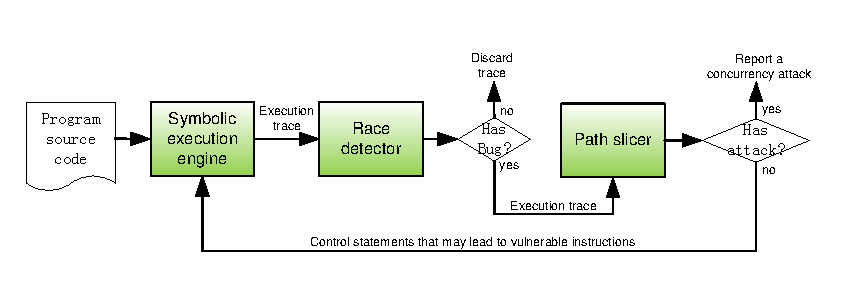
\includegraphics[width=.20\linewidth]{figures/detection}
% \label{fig:algo}}
% \vspace{-.05in}
% \caption{{\em \xxx's Concurrency Attack Detection Approach.}\label{fig:detect}
% \vspace{-.2in}
% \end{center}
% \end{figure}

\begin{figure}[!htb]
%     \centering
    \begin{minipage}{.5\textwidth}
%         \centering
        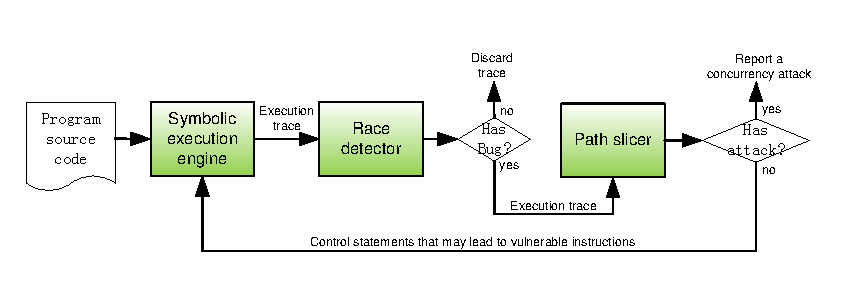
\includegraphics[width=0.34\textheight]{figures/detection}
        \vspace{0.1in}
        \caption{Workflow of detection approach. \\Three basic building blocks 
are shaded.}
        \label{fig:detection}
    \end{minipage}%
    \begin{minipage}{0.5\textwidth}
      \vspace{-.1in}
      \centering
      \begin{algorithm}[H]
      \DontPrintSemicolon
      \scriptsize
      \SetCommentSty{textrm}
      \SetKwInOut{Input}{Input}\SetKwInOut{Output}{Output}
      \Input{execuion trace $trace$, concurrency bug instructions $bug$}
      \Output{branch statements relevant to concurrency attacks}
      
      \SetKwBlock{Titlea}{Slicing($trace$)}{end}
      \Titlea {
        $slice$ $\leftarrow$ empty sequence \;
        \For {{\rm $i$ $\in$ reverse($trace$)}} {
          \If {{\rm $i$ $\in$ $bug$}} {
            {\bf break} \;
          }
          \If {{\rm any $e \in slice$ transitively depends on $i$}} {
            $slice$.push\_front($i$) \;
          }
          \ElseIf {{\rm $i$ is a branch instruction}} {
            \For {{\rm $j$ $\in$ instructions $i$ reaches off $trace$}} {
              \If {{\rm mayBeVulnerable($j$)}} {
                $slice$.push\_front($i$) \;
                {\bf break} \;
              }
            }
          }
        }
        \Return $slice$.branches() \;
      }
      \caption{Path slicing algorithm}
      \label{alg:slice}
      \end{algorithm}
    \vspace{-.1in}
    %     \caption{Sketch of path slicing algorithm}
%         \label{fig:algo}
\end{minipage}
\end{figure}



The path slicer is our core technique to track the propagation 
(\S\ref{sec:model}) from a concurrency bug to potential vulnerable instruction. 
The path slicer goes backward from the last execution of the trace and collects 
branch instructions that may lead to a vulnerable instruction in the 
not-executed branches. The path slicer then notifies symbolic execution to 
explore these branch instructions with high priority to increase the 
probability that following executions hit vulnerable instructions.

% P1: why need a detection scheme. First, capture as many as exploits in 
% testing phase. And call for re-install if there is any potential exploit. 
% Even for 
% old concurrency bugs, it is still necessary because exploits may have already 
% occured and attackers may have already broken in.

% P2: two research questions. Given a concurrency bug, will it lead to an 
% exploit?

% P3: if this bug may lead to an exploit, what inputs may lead to such exploits?

% P4: how to incorporate the patterns in previous section?

% P5: go over the workflow, which is a straight line of boxes. May add some 
% back edges to make it an iterative approach?
 
% \subsubsection{Implementing \xxx's Detection Scheme}\label{sec:detect-impl}
% TBD

% \vspace{-.15in}\subsubsection{Preliminary Results}
% \label{sec:detect-result}\vspace{-.075in}

% P1: we have implemented part of the dangerous operation. pointer NULL 
% derefence. Report the results. FP:FN. 
\para{Preliminary results.} We have developed two preliminary techniques for 
this detection approach. First, we have presented a precise path slicer called 
Woodpecker~\cite{woodpecker:asplos13} in in ASPLOS 2013 for detecting 
single-threaded security violations on system calls (\eg, \texttt{setuid()}). 
Woodpecker detects 113 programming rule violations in 136 popular systems 
programs, including seven serious ones already confirmed by developers. Second, 
we have also presented a data race detector in our 
and Peregrine~\cite{peregrine:sosp11} work in SOSP 2011. This race 
detector has detected several new data races in 
heavily-studied programs~\cite{wu:pldi12}.

% These preliminary results show the 
% feasibility of our proposed detection approach.

% P2: mention our initial work in OSDI '10 and SOSP '11 on precise data race 
% detection.


% P2: we foresee a few open challenges on the continuation of developing this 
% tool. First, how to make path slicing handle % non-function calls. Second, 
% how 
% to prioritize different operations ()? % Third, how to select malicious 
% inputs and thread schedules that are more likely to triger concurrency bugs?
\para{Open research challenges.} To guide the development of our detection 
approach, we foresee three open research challenges as our future development 
work. First, how to generalize our existing path slicing approach to support all the five types of 
vulnerable instructions we collected (\S\ref{sec:attack-phase})? Second, given the same 
type of a vulnerable instruction, how to enhance our path slicer to prioritize the more vulnerable ones other 
than the safe ones (\eg, some \texttt{strcpy()} functions are just 
manipulation on memory and do not involve inputs)? Third, how to guide our symbolic execution engine 
to explore malicious inputs and thread interleavings that are more likely to trigger concurrency 
bugs? We are confident that addressing each of these challenges will spur new 
significant techniques.

\vspace{-.15in}\subsection{Objective 3: Defending against Concurrency Attacks 
in Deployment Phase}\label{sec:defense}\vspace{-.075in}

% P1: motivation, why runtime detection is important. We want to mostly avoid 
% exploits by preventing attackers from manipulating the schedules.
Our detection approach proposed in \S\ref{sec:detect} is not 
designed to catch 100\% concurrency attacks because exploring 100\% program 
paths in symbolic execution is still an open research problem. Therefore, to 
practically prevent concurrency attacks taking over multi-threaded programs 
during the software deployment phase, this project proposes a runtime defense 
infrastructure.

% P2: reason 2: when races occur even if Parrot is enforced, we want to have 
% fault-tolerance.
Since a defense infrastructure requires tolerating failures of a program, 
this project plans to leverage \emph{state machine replication (or \smr)}, a 
powerful fault-tolerance concept in distributed systems. \smr 
models a program as a deterministic state machine, where the states are 
important program data and the transitions are deterministic executions of 
program code under input requests. SMR runs replicas of the program on 
different physical computers and invokes a distributed consensus protocol 
(typically \paxos~\cite{paxos,paxos:simple}) to ensure the same input sequence for replicas, 
as long as a majority of the replicas agrees on the sequence. 
Under the deterministic execution assumption, this majority of replicas must reach 
the same exact state despite various exceptions such as program failures. 
SMR is proven safe in theory~\cite{paxos,paxos:complex} and provides high availability in 
practice~\cite{chubby:osdi,zookeeper}.



% P3: reason 3: we want survive. checkpoint and re-execute, and diversify the 
% schedules before re-execute. Sell it like a self-healing runtime system.
Although \smr's fault-tolerant benefit makes it particularly attractive
on building a general runtime infrastructure for defending against 
concurrency attacks, we foresee four research challenges to realize this 
infrastructure. First, to leverage existing SMR systems such as 
ZooKeeper~\cite{zookeeper}, program developers have to shoehorn their programs into the 
narrowly defined state machine interfaces (\eg, ZooKeeper provides a file IO interface), 
a time-consuming and error-prone process.

Second, as introduced in \S\ref{sec:background}, even given the same 
input, multithreaded programs can easily run into too many different thread 
interleavings (or \emph{schedules}) at runtime depending on inter-thread 
communications (\eg, \mutexlock). Therefore, even if concurrency attacks do not 
manifest, different schedules can still easily cause replicas to diverge and no 
longer reach consensus. 


Third, if all replicas run into the same buggy schedules and trigger 
concurrency attacks, our infrastructure should automatically recover the 
replicas and make them switch to another schedules.

Fourth, in addition to regular synchronizations, our infrastructure should also 
handle various common ad-hoc synchronizations (\eg, to enforce an execution order, 
one thread does busy wait until a global variable is true, and another thread sets the 
variable to be true).

\vspace{-.15in}\subsubsection{Architecture of \xxx's Runtime Defense 
Infrastructure} 
\label{sec:defense-arch}\vspace{-.075in}

Figure~\ref{fig:defense} shows our proposed \smr-based infrastructure. This infrastructure 
addresses the first challenge by 
enabling a general multi-threaded program run in it \emph{transparently} 
without modifications. A major benefit of transparency is that program 
developers can focus on implementing their program's functionality, not how to 
defend against concurrency attacks.

To achieve transparency, within each \smr replica, this 
infrastructure interposes on the socket and the thread synchronization 
interfaces to keep replicas in sync. Specifically, it considers each incoming socket call (e.g., \texttt{accept()} a 
client's connection or \texttt{recv()} a client's data) an input request, and 
runs a \paxos consensus protocol to ensure that a majority of the replicas sees 
the same exact sequence of the incoming socket calls.

% \begin{figure}[t]
% \centering
% 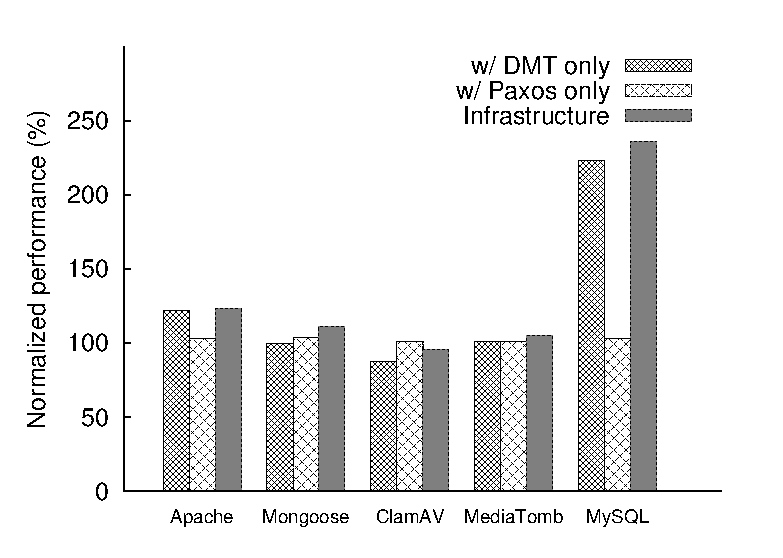
\includegraphics[width=0.5\textwidth]{figures/normalize-perf}
% \vspace{-.30in}
% \caption{\small {\em \xxx's performance normalized to un-replicated 
% nondeterministic execution.}}
% \label{fig:normalize-perf}
% \end{figure}

% \begin{figure}[ht]
% \centering
% \vspace{-.1in}
% 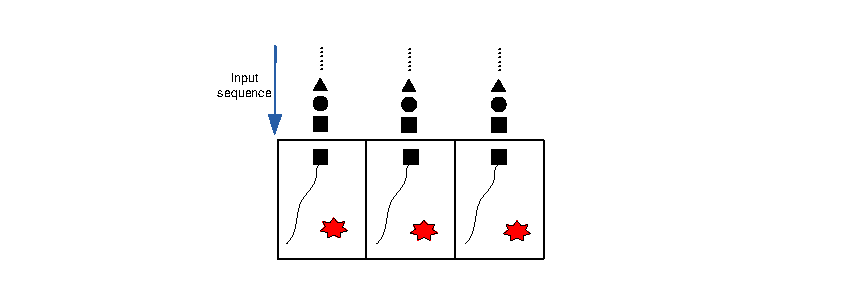
\includegraphics[width=0.35\columnwidth]{figures/defense}
% \vspace{-.1in}
% \caption{{A runtime infrastructure to defend against concurrency attacks.}} 
% \label{fig:defense}
% \vspace{-.15in}
% \end{figure}


\begin{figure}[!htb]
    \centering
    \begin{minipage}{0.5\textwidth}
%       \centering
       \hspace{.25in}
%        \vspace{0.3in}
      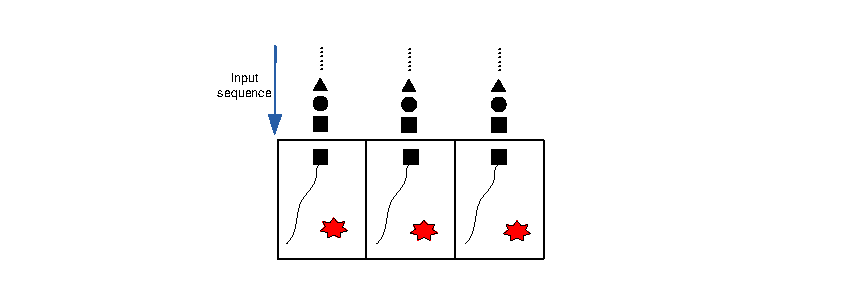
\includegraphics[width=0.25\textheight]{figures/defense}
       \vspace{-.02in}
      \caption{{Defense infrastructure. Solid shapes \\
      are inputs; curve lines are schedules.}} 
      \label{fig:defense}
    \end{minipage}%
    \begin{minipage}{0.5\textwidth}
%       \centering
%       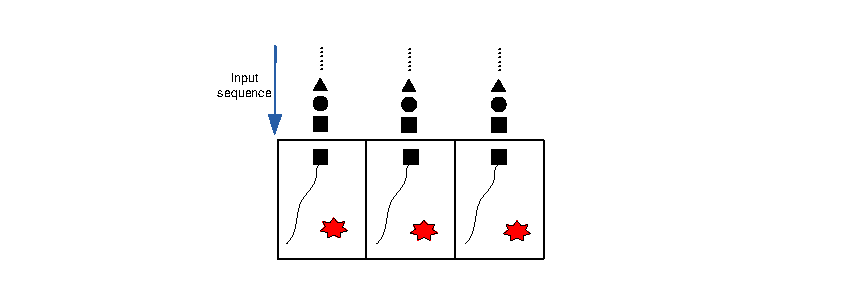
\includegraphics[width=0.35\columnwidth]{figures/defense}
       \vspace{-.3in}
      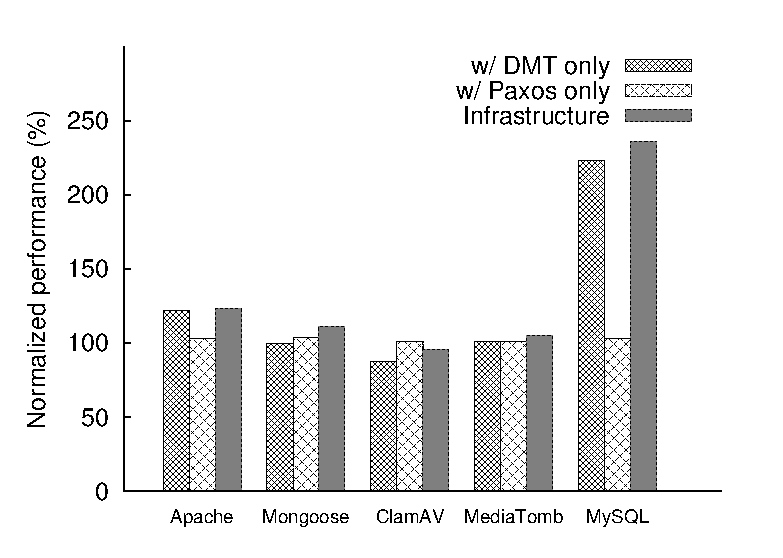
\includegraphics[width=0.35\textheight]{figures/normalize-perf.eps}
      \vspace{-.15in}
      \caption{{The infrastructure's performance normalized to 
programs' native execution.}}
      \label{fig:normalize-perf}
    \end{minipage}
      \vspace{-.2in}
\end{figure}



To address the second challenge, this infrastructure schedules synchronizations 
using \emph{deterministic 
multithreading (\dmt)}~\cite{dpj:oopsla09,dmp:asplos09,kendo:asplos09,
coredet:asplos10, 
dos:osdi10,ddos:asplos13,ics:oopsla13}.  This technique typically maintains a 
\emph{logical time}, that advances deterministically on each thread's 
synchronization. By serializing thread synchronizations with a specific policy 
(\eg, round-robin or first-come-first-serve), \dmt practically makes an entire 
multithreaded execution deterministic. The overhead of \dmt is typically 
moderate because most code is not synchronization and can still run in parallel.


% \begin{figure}[ht]
% \centering
% 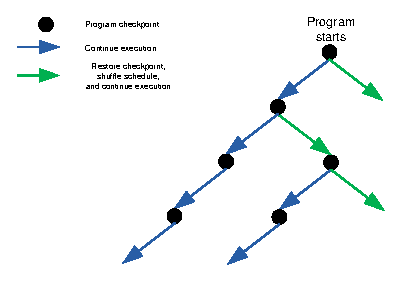
\includegraphics[width=0.3\columnwidth]{figures/healing}
% \vspace{-.05in}
% \caption{{The self-healing idea for recovering from concurrency attacks.}} 
% \label{fig:healing}
% \vspace{-.05in}
% \end{figure}

% Mention the self healing idea.
To address the third challenge, we plan to leverage recent 
Linux process checkpoint/restore techniques, including process state (\eg, 
memory)~\cite{criu} and file system state~\cite{lxc}. Our each 
checkpoint operation will be done on a backup replica (see 
Figure~\ref{fig:defense}) so that it will not affect the other replicas to 
efficiently reach consensus on inputs and send responses. To handle all replicas 
running into the same buggy schedules (buggy schedules are extremely rare 
compared to correct schedules~\cite{lu:concurrency-bugs}), we will develop an 
"observer" program that runs on a dedicated machine to periodically check the 
status of replicas. If a majority of replicas fails, the observer restarts all 
replicas, restores program state on replicas with the latest checkpoint, and 
enforces a different \dmt policy.
% If minor replicas fail, \smr's 
% fault-tolerance strength still makes the other replicas run.

To address the fourth challenge, we plan to leverage recent advances on 
automatically annotating ad-hoc synchronizations~\cite{syncfinder:osdi10, 
cfix:osdi12}, and then we leverage a \dmt scheduler (\eg,~\cite{dthreads:sosp11, 
parrot:sosp13}) to schedule these ad-hoc synchronizations in a deterministic 
order.

% As a typical security setting, we need to define which components of 
% this Infrastructure must be trusted. In this project, we require the 
% infrastructure and the checkpoints are trusted (\ie, even if the program 
% compromises, its program checkpoints and the infrastructure are not effected). 
% We consider this requirement as reasonable, because once this infrastructure is 
% built, we can leverage existing verification techniques to focus on verifying 
% this infrastructure, and on top of it, we no longer need to verify those 
% programs.




% P4: challenges on doing so. Including the initial work.



% To address the third and fourth challenges, 
% this infrastructure schedules synchronizations 
% using deterministic multithreading (DMT). This technique typically maintains a 
% global, monotonically increasing logical clock that advances deterministically 
% on each thread's synchronization. By serializing thread synchronizations, DMT 
% practically makes an entire multithreaded execution deterministic. The overhead
% of DMT is typically moderate because most code is not synchronization and can 
% still run in parallel.

\vspace{-.15in}\subsubsection{Preliminary Results} 
\label{sec:defense-result}\vspace{-.075in}

% P1: we have built a replication system. Perf and checkpoint results.
We have developed preliminary systems to address the first two challenges. To 
address the first challenge, we have built a transparent \smr system 
\crane~\cite{crane:sosp15}. \crane is able to transparently support five widely 
used server programs, with 34.2\% overhead in average (see 
Figure~\ref{fig:normalize-perf}). To address the second challenge, we have built 
an efficient \dmt runtime \parrot~\cite{parrot:sosp13}, which incurred merely 
12.7\% overhead on a wide range of 108 popular multithreaded programs on 24-core 
machines.

\vspace{-.15in}\subsection{Research Plan} \label{sec:plan}\vspace{-.075in}

This project will require two PhD students S1 and S2 for a period of 
three years. In the first year, S1 will develop and refine the concurrency 
attack model (part of \textbf{Objective 1}), and S2 will leverage the model to 
design the detailed workflow of the detection approach (part of \textbf{Objective 2}) by working 
closely with S1. In the second year, S1 will do an empirical study on how well 
the model represents real-world concurrency attacks (part of \textbf{Objective 1}), and S2 will implement 
the detection approach as a software tool (part of \textbf{Objective 2}). In the third 
year, S1 will build the defense infrastructure (\textbf{Objective 3}), and S2 
will study the detection tool on broad real-world programs to find new attacks.
% Both students will 
% involve theoretical methods, implement real software systems, and 
% perform real-world study.
% The PI will supervise the students by providing 
% advice concerning both theoretical and systems implementation levels.


